\documentclass{beamer}
\usetheme{default}
%\usetheme{pittsburgh}
\usecolortheme{albatross}

%###############################################################################
%#
%# Saját színek:
%#
\definecolor{todobgszin}{rgb}{0.64000,0.78000,0.22000}
\definecolor{todofrszin}{rgb}{0.00000,0.50000,0.00000}
\definecolor{background}{rgb}{0.00000,0.29412,0.49804}
%#
%###############################################################################

\setbeamercolor{normal text}{fg=white}
\setbeamertemplate{navigation symbols}{} % Navigációs ikonok off

\usepackage[T1]{fontenc}
\usepackage[utf8]{inputenc}
\usepackage[english,magyar]{babel}

\usepackage{hyperref}
\usepackage{color}
\usepackage{graphics}

\usebackgroundtemplate{

\includegraphics[width=\paperwidth, height=\paperheight]{figures/background.jpg}
}

% Néhány konstans deklarációja:
\newcommand{\vikszerzo}{Nádudvari György}
\newcommand{\vikszerzomail}{ulqp9p@gmail.com}
\newcommand{\vikkonzulens}{Huszerl Gábor}
\newcommand{\vikcim}{Oktatástámogató rendszerek kiszolgáló infrastruktúrájának felügyeleti lehetőségei}

%###############################################################################
%#
%# Footer definíció a szokásos címek beírásához.
%#
%# Csúnya hacket tartalmaz!!!
%# A "{footline}{#1}" utáni \textcolorral egy háttérszínnel megegyező "y"
%# karaktert írunk ki, hogy ne ugráljanak a dobozok a diákon.
%# Ha ez elmarad, akkor az alapvonal alá nyúló karaktereket (pl. g, y stb.)
%# tartalmazó stringek esetén eltérő magasságban lesz a footer, mint azoknál
%# amelyek csak az alapvonalra illeszkedő karaktereket tartalmaznak.
%#
\newcommand{\setfootline}[1]{\setbeamertemplate{footline}{\setbeamercolor{footline}{fg=white}\begin{beamercolorbox}[sep=1cm,wd=\textwidth,ht=1cm,left]{footline}{#1}\textcolor{background}{y}\end{beamercolorbox}}}
%#
%###############################################################################

%###############################################################################
%#
%# Saját eszközök:
%#
\newcommand{\todo}[1]{\fcolorbox{todofrszin}{todobgszin}{\emph{TODO: #1}}}
\newcommand{\angolul}[1]{\foreignlanguage{english}{#1}}
%#
%###############################################################################

\hypersetup{
    bookmarks=true,            % show bookmarks bar?
    unicode=true ,             % non-Latin characters in Acrobat’s bookmarks
    pdftitle={\vikcim},        % title
    pdfauthor={\vikszerzo},    % author
    pdfcreator={\vikszerzo},   % creator of the document
    pdfnewwindow=true,         % links in new window
    colorlinks=true,           % false: boxed links; true: colored links
    linkcolor=black,           % color of internal links
    citecolor=black,           % color of links to bibliography
    filecolor=black,           % color of file links
    urlcolor=black             % color of external links
}

\title{\vikcim}
\author{\vikszerzo \\ \footnotesize{\texttt{\vikszerzomail}} \\[0.5cm] \normalsize{Konzulens: \vikkonzulens}}
\date{2012. június 14.}

\begin{document}

\section{\vikcim}
\begin{frame}[plain]
\titlepage
\end{frame}

\section{Miről is lesz szó?}
\setfootline{Interstellar Overdrive}
\begin{frame}[t]
\frametitle{Miről is lesz szó?}
\begin{itemize}
    \item Tanulásmenedzsment rendszerek
        \begin{itemize}
            \item fogalma, feladatai
            \item átjárhatóság közöttük és miért fontos ez
        \end{itemize}
    \item Tanulásmenedzsment rendszerek IT infrastruktúrája
        \begin{itemize}
            \item A három rétegű architektúra a Moodle rendszeren bemutatva
        \end{itemize}
    \item Tanulásmenedzsment rendszerek erőforrás igényei
        \begin{itemize}
            \item Alapvető igények
            \item Modellek
        \end{itemize}
    \item Információs technológiai infrastruktúrák
        \begin{itemize}
            \item A klasszikus IT infrastruktúra
            \item Felhőalapú infrastruktúrák
        \end{itemize}
    \item IT infrastruktúrák proaktív menedzsmentje általános és oktatástámogató rendszerek esetén
    \item Összefoglalás
\end{itemize}
\end{frame}

\section{Tanulásmenedzsment rendszerek}
\setfootline{Remember a Day}
\begin{frame}[t]
\frametitle{Mik azok a tanulásmenedzsment rendszerek?}
\begin{itemize}
    \item Milyen rendszereket nevezünk \angolul{Learning Management Systemnek} (LMS-nek)?   
    \item Mik egy LMS feladatai?   
    \item Milyen megoldásokat találunk a piacon?   
    \item Miért fontos az átjárhatóság?  
    \item Mi az a SCORM, és mire jó?
\end{itemize}
\end{frame}

\section{LMS-ek IT infrastruktúrája}
\setfootline{\angolul{Pigs (Three Different Ones)}}
\begin{frame}[t]
\frametitle{LMS-ek IT infrastruktúrája}
\begin{figure}[!ht]
\centering
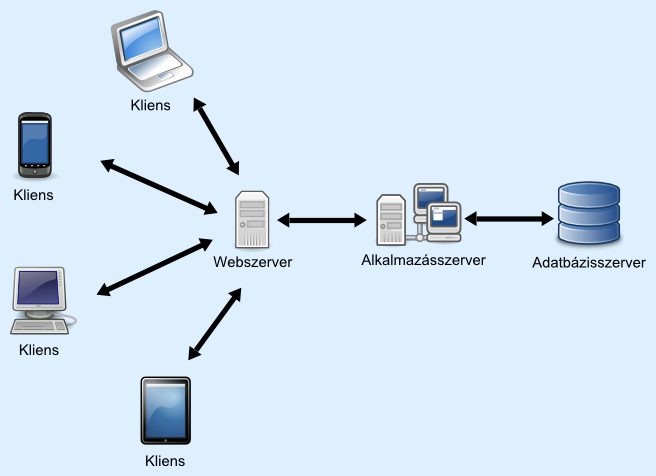
\includegraphics[width=90mm, keepaspectratio]{figures/3tier_simple_001.png}
\end{figure}
\end{frame}

\section{LMS-ek IT infrastruktúrája - Megvalósítás}
\setfootline{\angolul{Pigs on the Wing}}
\begin{frame}[t]
\frametitle{LMS-ek IT infrastruktúrája - Megvalósítás}
\begin{figure}[!ht]
\centering
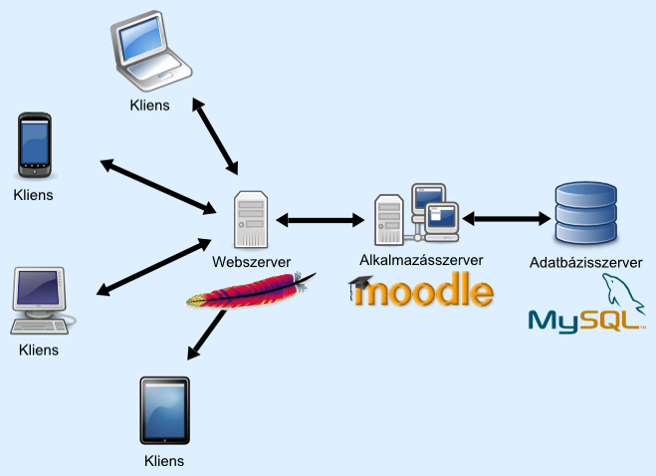
\includegraphics[width=90mm, keepaspectratio]{figures/3tier_simple_001_with_logos.png}
\end{figure}
\end{frame}

\section{Tanulásmenedzsment rendszerek erőforrás igényei}
\setfootline{\angolul{A New Machine}}
\begin{frame}[t]
\frametitle{Tanulásmenedzsment rendszerek erőforrás igényei}
\begin{itemize}
    \item Alapvető igények
    \begin{itemize}      
        \item Webszerverek erőforrásigénye        
        \item Adatbázisszerverek erőforrásigénye
    \end{itemize}
    \item Modellek
    \begin{itemize}       
        \item Lehetséges felhasználói viselkedéssel kapcsolatos és statisztikai modellek alkotása
    \end{itemize}
\end{itemize}
\begin{figure}[!ht]
\centering
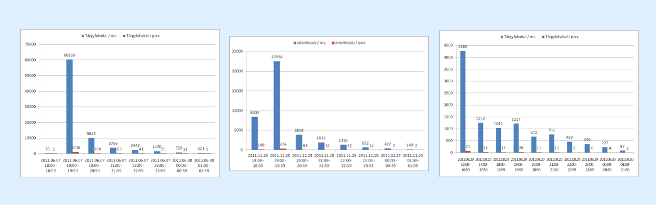
\includegraphics[width=110mm, keepaspectratio]{figures/modellek.png}
\end{figure}
\end{frame}

\section{Információs technológiai infrastruktúrák}
\setfootline{\angolul{Any Colour You Like}}
\begin{frame}[t]
\frametitle{Információs technológiai infrastruktúrák}
\begin{itemize}
    \item A klasszikus IT infrastruktúra
    \begin{itemize}
        \item Adatbázis réteg
        \begin{itemize}           
            \item terheléselosztás (load balancing)
            \item replikálás
            \item feladatátadás hiba esetén (failover) 
        \end{itemize}
        \item Alkalmazás réteg
        \item Webkiszolgáló réteg
    \end{itemize}
    \item Virtualizáció
    \item Felhőalapú infrastruktúrák
\end{itemize}
\end{frame}

\section{Felhőalapú infrastruktúrák az LMS-ek szemszögéből}
\setfootline{\angolul{The Great Gig in the Sky}}
\begin{frame}[c]
\frametitle{Felhőalapú infrastruktúrák az LMS-ek szemszögéből}
\begin{figure}[!ht]
\centering
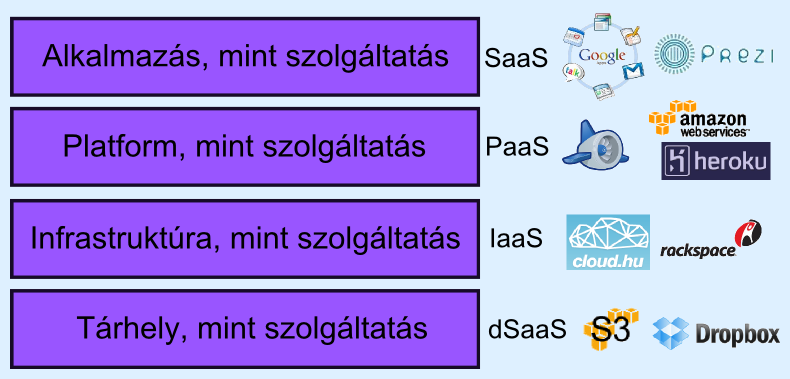
\includegraphics[width=90mm, keepaspectratio]{figures/cloud_service_models.png}
\end{figure}
\end{frame}

\section{IT infrastruktúrák proaktív menedzsmentje általános és oktatástámogató rendszerek esetén}
\setfootline{\angolul{Welcome to the Machine}}
\begin{frame}[t]
\frametitle{IT infrastruktúrák proaktív menedzsmentje általános és oktatástámogató rendszerek esetén}
Egy IT infrastruktúra (de valójában bármilyen rendszer) menedzsmentje lehet:
\begin{itemize}
\item reaktív
\item proaktív
\end{itemize}
\end{frame}

\section{IT infrastruktúrák menedzsmentje reaktív esetben}
\setfootline{\angolul{Let There Be More Light}}
\begin{frame}[c]
\frametitle{IT infrastruktúrák menedzsmentje reaktív esetben}
\begin{figure}[!ht]
\centering
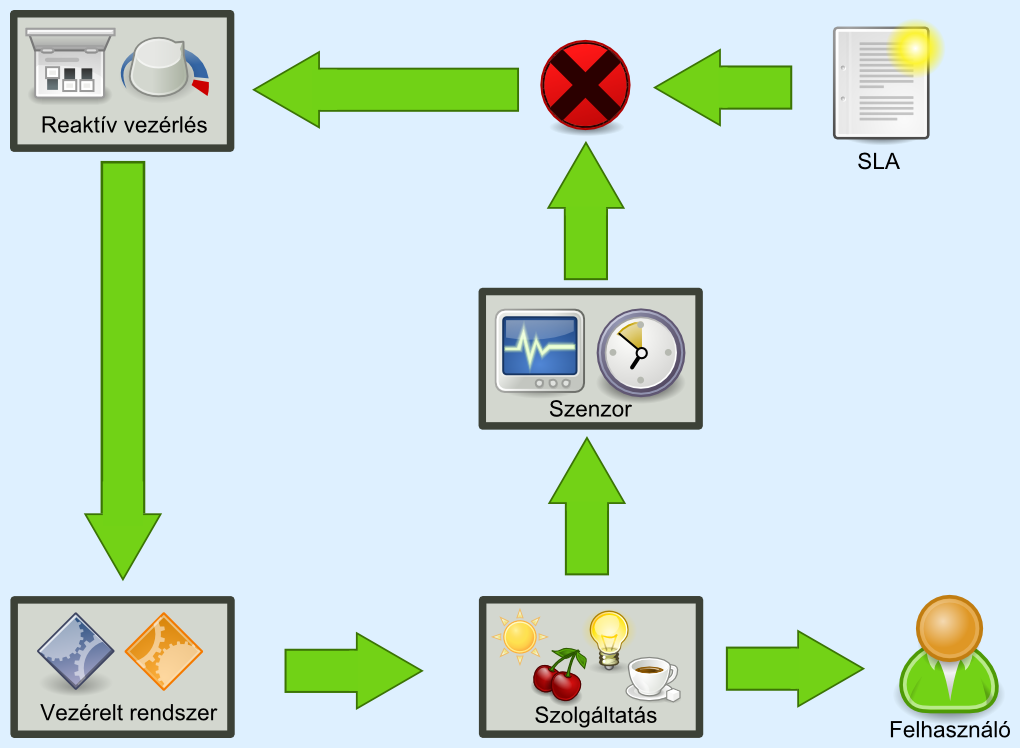
\includegraphics[width=90mm, keepaspectratio]{figures/reactive_system.png}
\end{figure}
\end{frame}

\section{IT infrastruktúrák menedzsmentje proaktív esetben}
\setfootline{\angolul{Set the Controls for the Heart of the Sun}}
\begin{frame}[c]
\frametitle{IT infrastruktúrák menedzsmentje proaktív esetben}
\begin{figure}[!ht]
\centering
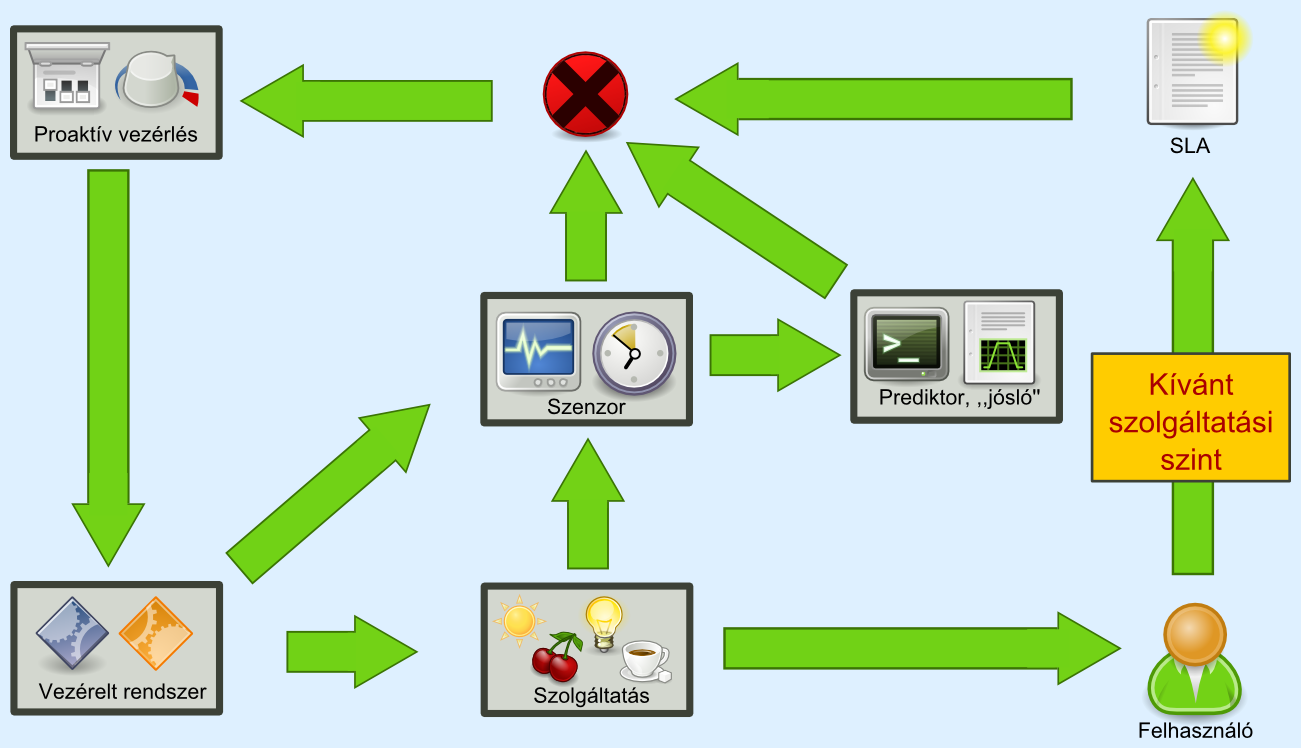
\includegraphics[width=110mm, keepaspectratio]{figures/proactive_system.png}
\end{figure}
\end{frame}

\section{Hogyan kerül a csizma proaktívan az asztalra?}
\setfootline{\angolul{If}}
\begin{frame}[t]
\frametitle{Hogyan kerül a csizma proaktívan az asztalra?}
LMS-ek esetében is alkalmazható menedzsment:
\begin{itemize}
\item ha modellek segítségével jósolható a felhasználók viselkedése,
\item ha az LMS lehetőséget biztosít az alkalmazási rétegből a többi réteg működésébe való beavatkozásra
\item ha az infrastruktúránk (saját rendszer, felhőalapú megvalósítás) lehetőséget biztosít a beavatkozásra 
\end{itemize}
Lehetséges megvalósítási példa:
\begin{itemize}
\item Moodle teszt létrehozása esetén automatikusan erőforrások hozzáadása a rendszerhez az Amazon API-jának megfelelő metódusainak meghívásával
\end{itemize}
\end{frame}

\section{Összefoglalás}
\setfootline{\angolul{Breathe}}
\begin{frame}[t]
\frametitle{Összefoglalás}
Bemutattam
\begin{itemize}
\item az LMS-ek fogalmát,
\item erőforrás igényeiket, és azok változásainak okait,
\item az LMS-ek üzemeltetésének előnyeit cloud rendszerekben.
\end{itemize}
Felvetettem
\begin{itemize}
\item az erőforrás igények változásainak felügyeleti lehetőségeit proaktív menedzsment esetén,
\item erre egy lehetséges implementációs megoldást.
\end{itemize}
\end{frame}

\section{A bíráló kérdése}
\setfootline{\angolul{The Trial}}
\begin{frame}[t]
\frametitle{A bíráló kérdése}
\textbf{Kérdés}:
\begin{itemize}
\item Hogyan specifikálná (vagy hogyan véleményezné) azokat az intézményi igényeket (szerzői jogok, biztonsági szempontok, stb.) amikor már nem javasolt az LMS futtatása a felhőalapú infrastruktúrán?
\end{itemize} 
\textbf{Válasz}:
\begin{itemize}
\item Léteznek kezdeményezések, megoldások a problémára
\end{itemize}
\end{frame}

\section{Kérdések}
\setfootline{\angolul{Is There Anybody Out There?}}
\begin{frame}[c]
\frametitle{}
\begin{center}
\huge{\textbf{Kérdések?}}\\
\begin{figure}[!ht]
\centering

\includegraphics[width=20mm, keepaspectratio]{figures/questions.png}
\end{figure}
\end{center}
\end{frame}

\section{Vége}
\setfootline{\angolul{Comfortably Numb}}
\begin{frame}[c]
\frametitle{}
\begin{center}
\huge{\textbf{Köszönöm a figyelmet!}}
\end{center}
\end{frame}

\end{document}
